\documentclass[UTF8]{ctexart}
\usepackage[colorlinks,linkcolor=blue]{hyperref}%超链接
\usepackage{gensymb}%°
\usepackage{newtxtext, newtxmath}%两行用来设置timesnewRome
\usepackage{graphicx} %图片控制宏包;使用\caption{} 为图片添加名称。
\usepackage{bm} %公式字母加粗
\usepackage{subfigure}%用于插入多张图片
\usepackage{amsmath}
\usepackage{physics}
\usepackage{mathrsfs}%花体字符:调用$\mathbb{R}$
\usepackage{graphicx}
\usepackage{subfigure}
\usepackage{color}
\usepackage{ulem}%下划线\uline{text}
\usepackage{comment}

\graphicspath{{./figure/}}%路径
\DeclareGraphicsExtensions{.pdf, .jpeg, .png, .jpg}

\begin{document}
\section{第5章 光学全息}
\subsection{全息光学概述}
\subsection{波前记录与再现}
\subsubsection{波前记录}
\begin{figure}[htbp]
    \centering
    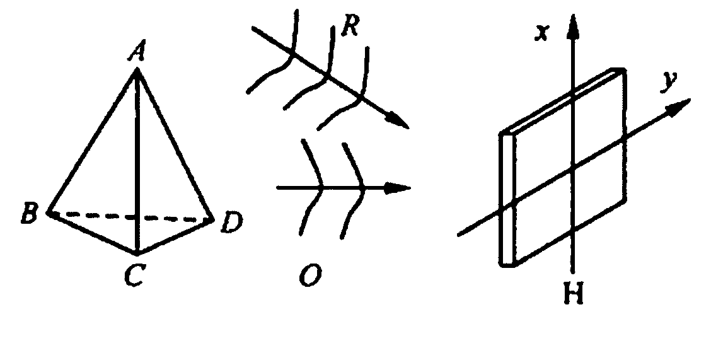
\includegraphics[width=0.7\textwidth]{1.PNG}
    \caption{波前记录}
    \label{1}
\end{figure}
\begin{enumerate}
    \item 用干涉方法记录物光波波前

    必须设法把相位信息转换成强度变化才能记录。干涉法是将空间相位调制转换为空间强度调制的标准方法。

    物光波为
    \begin{equation}
        {O}\left( {x,y} \right) = \left|O\left( {x,y} \right)\right|\exp \left[ { - j\varphi \left( {x,y} \right)} \right],
    \end{equation}
    参考光为
    \begin{equation}
        {R}\left( {x,y} \right) = \left|R\left( {x,y} \right)\right|\exp \left[ { - j\psi \left( {x,y} \right)} \right],
    \end{equation}
    总光强为
    \begin{equation}
        \begin{aligned}
                I\left( {x,y} \right) &= {\left| {R\left( {x,y} \right) + O\left( {x,y} \right)} \right|^2}\\
                 &= {\left| {R\left( {x,y} \right)} \right|^2} + {\left| {O\left( {x,y} \right)} \right|^2} + R\left( {x,y} \right){O^*}\left( {x,y} \right) + {R^*}\left( {x,y} \right)O\left( {x,y} \right)
        \end{aligned}
    \end{equation}
    或者
    \begin{equation}
        I\left( {x,y} \right) = {\left| {R\left( {x,y} \right)} \right|^2} + {\left| {O\left( {x,y} \right)} \right|^2} + 2\left| {R\left( {x,y} \right)} \right|\left| {O\left( {x,y} \right)} \right|\cos \left[ {\psi \left( {x,y} \right) - \varphi \left( {x,y} \right)} \right].
    \end{equation}
    \item 记录过程的线性条件
    \begin{figure}[htbp]
        \centering
        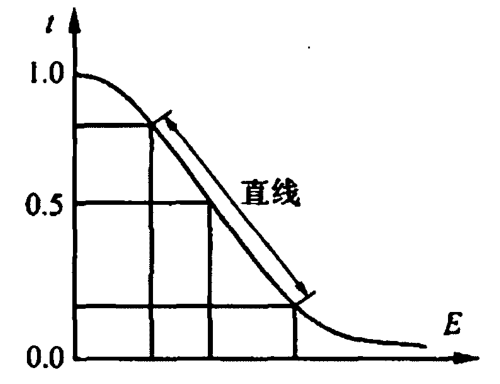
\includegraphics[width=0.7\textwidth]{2.PNG}
        \caption{负片的$t-E$曲线}
    \end{figure}
    假定全息干板是一个线性变换器,并且有足够高的分辨率,以便能记录全部入射的空间结构。则其振幅透过率为
    \begin{equation}
        t\left(x,y\right)=t_0+\beta E = t_0 + \beta\left[\tau I\left(x,y\right)\right] = t_0 + \beta'I\left(x,y\right).
    \end{equation}
    其中$\beta'$为曝光时间$\tau$和斜率$\beta$的乘积,对于负片和正片$\beta'$分别为负值和正值。假设参考光的强度在整个记录表面是均匀的,那么
    \begin{equation}
        t\left( {x,y} \right) = {t_0} + \beta '\left( {{{\left| R \right|}^2} + {{\left| O \right|}^2} + R{O^*} + {R^*}O} \right) = {t_b} + \beta '\left( {{{\left| O \right|}^2} + R{O^*} + {R^*}O} \right).
    \end{equation}
    其中$t_b=t_0+\beta'\left|R\right|^2$,表示均匀偏置透过率。
\end{enumerate}
\subsubsection{波前再现}
\begin{enumerate}
    \item 衍射效应再现物波波前

    假设落在全息图平面上的复振幅为$C\left(x,y\right)$,则透过全息图的光场为

    \begin{equation}
        \begin{aligned}
            U\left( x,y \right)&=C\left( x,y \right)t\left( x,y \right)=t_bC + \beta'OO^*c + \beta'R^*CO + \beta'RCO^* \\&= U_1 + U_2 +U_3 +U_4.
        \end{aligned}
    \end{equation}

    其中我们将$C$、$O$、$O^*$视为波前函数,他们各自的系数视为一种波前变换或一种运算操作。如果系数含有二次相位,则相当于波前经过了一个透镜聚散;如果系数中出现了线性因子,则相当于波前经过了一个棱镜的偏转;如果两者兼有,则说明经过了棱镜和透镜。
    \begin{enumerate}
        \item $U_1$系数$t_{b}=t_0+\beta'R^2$,其中参考光常用平面波或简单的球面波,近似常数;
        \item $U_2$系数含有$O^{2}$,代表振幅受到调制的照明波前,也就是$C$波经历$O^2\left( x,y \right)$分布的底片的衍射,适当调整照明度,可以使其成为次要因素;

        \uline{以上两个分量基本保留了照明光的特性,成为全息图衍射场的\textbf{0级波}}
        \item 当照明光波与参考光波完全相同$C=R$时,
        \begin{equation}
            U_3\left( x,y \right) = \beta'\left|R\right|^2O\left( x,y \right),
        \end{equation}$U_3$系数除了相差常数因子$R^2$外,是物光波的准确再现,并且由于原始物光波是发散的,所以是物体的\textbf{虚像},此称为全息图衍射场中的\textbf{$+1$级波};
        \item 当照明光波与参考光波完全相同$C=R$时,
        \begin{equation}
            U_4\left( x,y \right) = \beta'R^2O\left( x,y \right),
        \end{equation}
        此时$R^2$中的相位因子一般无法消除,此项称为全息图衍射场中的\textbf{$-1$级波}。

        只有当照明光波与参考光均为正入射平面波时,此时$\pm1$级光波才严格镜像对称,此时共轭光产生的实像对于观察者而言凹凸与原物体正好相反,称为\textbf{赝像}。
    \end{enumerate}
    \begin{figure}[htbp]
        \centering
        \subfigure[用原始参考波照明]{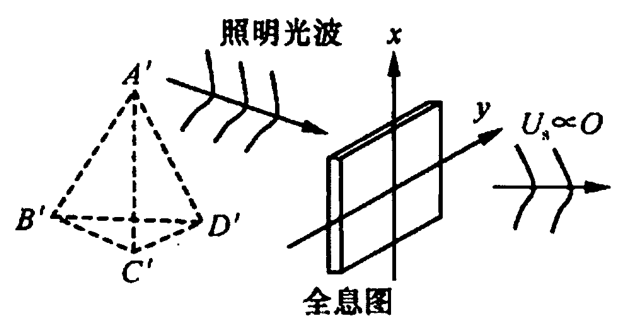
\includegraphics[width=0.45\textwidth]{3_1.PNG}}
        \subfigure[用共轭参考波照明]{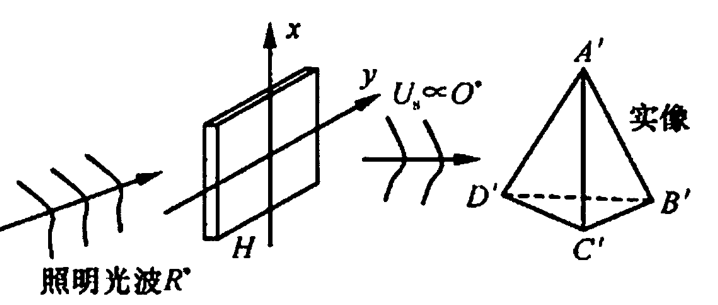
\includegraphics[width=0.45\textwidth]{3_2.PNG}}
        \caption{波前再现}
    \end{figure}
    \item 波前再现过程的线性性质

    \begin{itemize}
        \item 若把波前记录和波前再现的过程视为一种系统变换,那么记录的物波场为输入,再现波场为输出,这样的系统实现的变换是高度非线性的。
        \item 若把记录的物波前视为输入,再现时的投射场的单项分量作为输出,那么对应系统就是线性系统。
    \end{itemize}
     
\end{enumerate}

\subsubsection{全息图的基本类型}

\begin{itemize}
    \item 物光和参考光是否同轴:同轴全息、离轴全息;
    \item 物体与全息图片的相对位置:菲涅尔全息图、像面全息图、傅里叶变换全息图;
    \item 记录介质的厚度:平面全息图、体积全息图。
\end{itemize}

\subsection{同轴全息图和离轴全息图}
\subsubsection{同轴全息图}
\begin{figure}[htbp]
    \centering
    \subfigure[记录]{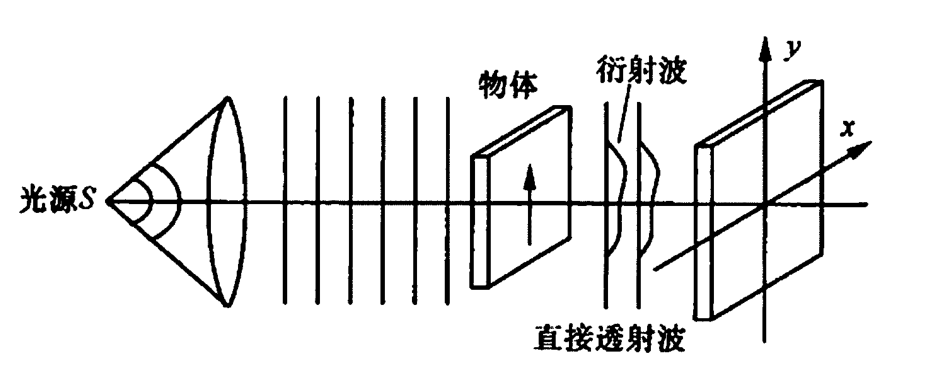
\includegraphics[width=0.45\textwidth]{4_1.PNG}}
    \subfigure[再现]{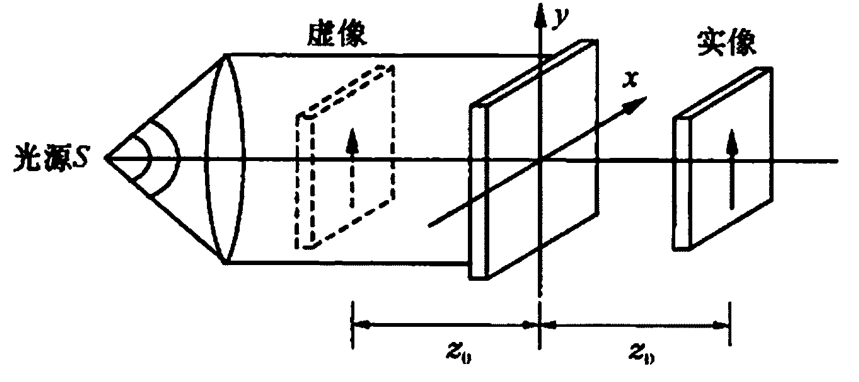
\includegraphics[width=0.45\textwidth]{4_2.PNG}}
    \caption{同轴全息图的记录与再现}
\end{figure}
假设相干平面波照明一个\textbf{高度透明}的物体,透射光场可以表示为
\begin{equation}
    t\left( x_0,y_0 \right) = t_0 + \Delta t \left( x_0,y_0 \right),
\end{equation}
其中,$t_0$是一个很高的平均透射率,$\Delta t$表示围绕平均值的变化,$\left|\Delta t\right|\le\left|t_0\right|$。

透射光场可以看做两项组成:
\begin{itemize}
    \item 由$t_0$表示的、强而均匀的平面波,相当于波前记录时的参考波;
    \item 有$\Delta t$表示的弱散射波,相当于波前记录时的物光波。
\end{itemize}

在距离物体距离$z_0$处防止全息图干板时曝光光强为
\begin{equation}
    I\left( x,y \right) = \left|R + O \left( x,y \right)\right|^2 = \left|R\right|^2 + \left|O\left( x,y \right)\right|^2 + R^*O\left( x,y \right) + RO^*\left( x,y \right).
\end{equation}

线性记录条件下,全息图振幅透过率正比于曝光光强
\begin{equation}
    t\left( x,y \right) = t_b + \beta'\left( \left|O\right|^2 + R^*O + RO^* \right).
\end{equation}

若用振幅为$C$的平面波垂直照明全息图,则透射光场可用四项场分量之和表示为
\begin{equation}
    U\left( x,y \right) = Ct\left( x,y \right) = Ct_b
     + \beta'C\left|O\left( x,y \right)\right|^2 + \beta'R^*CO\left( x,y \right) + \beta'RCO^*\left( x,y \right).
\end{equation}
\begin{itemize}
    \item 第一项是均匀衰减的平面波;
    \item 第二项正比于弱的散射光的光强,可以忽略不计;
    \item 第三项正比于$O\left( x,y \right)$,再现原始物光波前,产生原始物体的一个虚像;
    \item 第四项正比于$O^*\left( x,y \right)$,在虚像对称位置产生物体的实像。
\end{itemize}
特点:
\begin{itemize}
    \item 四项场分量都在同一方向上传播;
    \item 直接透射光降低了像的衬度;
    \item 虚像实像构成不可分离的孪生像,降低了全息像的质量;
    \item 最大局限:必须假定物体是高度透明的,否则第二项场分量将不可忽略。
\end{itemize}

\subsubsection{离轴全息图}
\end{document}
